\section{Longest Common Subsequence (LCS) } \label{lcs}
Another widely used metrics in the time-series similarity is the Longest Common Subsequence or LCS. LCS could be seen as the successor of the application of the Euclidean distance, DTW or scales and shifts \cite{citeulike:3816327} since it might be essentially based on any of these. 
\begin{figure}[tbp]
   \centering
   \includegraphics[height=40mm]{lcs.eps}
   %%{seriesheatmap}
   \caption{This figure is taken from \cite{citeulike:4367061} and while it designed to explain LCS application to the sequences of images it easily explains any of LCS and feature decomposition based approach to time-series similarity.}
   \label{fig:lcs}
\end{figure} 
The idea of LCS is explained in the classical Computer Science manuscript \cite{citeulike:180287} (CLR) for the string matches with use of the Dynamic Programming and have the complexity of $O(NM)$. 

Yazdani and Ozsoyoglu in \cite{citeulike:4367061} proposed new algorithm with better complexity $O(N+M)$ specifically for image sequences generalizing it further for any real-valued signals and specifically pointed application to time-series represented by the set of features like Fourier coefficients, etc. The Figure \ref{fig:lcs} taken from the article explains the approach taken: each of the images is approximated by the set of the specific to the domain real-values, and if $R$ and $S$ match then $FR$ and $FS$ match analogously, if $FR$ and $FS$ are similar then $R$ and $S$ are similar.

\begin{figure}[bp]
   \centering
   \includegraphics[height=100mm]{agrawal.eps}
   %%{seriesheatmap}
   \caption{This figure is taken from \cite{citeulike:3816327} and explains the modified LCS application for the sequence matching.}
   \label{fig:agrawal_lcs}
\end{figure} 

Algorithm starts with two sequences $X$ and $Y$ with lengths $N$ and $M$ respectively and building the vector data structure $C_{vect}$ of the size of the shorter one such that $C_{vect}[i]$ is the index of the element in $Y$ which matches with $i$th element of $X$. By letting $C[i,j]$ to be the length of the longest common subsequence of $X_{i}$ and $Y_{i}$ they define it as 

\begin{equation}
 C[i,j] = 
 \begin{cases} 
  0 \; \text{if } i=0 \; \text{or} \; j=0 \\
  C[i-1,j-1]+1 \; \text{if } i,j>0 \; \text{and } x_{i} \; \text{matches } y_{i} \\
  \max{C[i,j-1], \;C[i-1,j]} \; \text{otherwise}
 \end{cases}
\label{eq:lcs}
\end{equation}

By modifying the range of matching in the definition \ref{eq:lcs} to the specific (relaxed) bounds they achieved a better performance being able to improve the sensitivity of the method. 

Agrawal et al. \cite{citeulike:3816327}, as mentioned before, introduced LCS-based concept of similarity with local scaling, shifting and deletions, measuring the similarity based on the amount of non-overlapping time-ordered pairs of subsequences that are similar instead of individual points as displayed at the Figure \ref{fig:agrawal_lcs}. The complexity of LCS algorithm is $O(NM)$.